\documentclass{article}
\usepackage{tikz}

\begin{document}

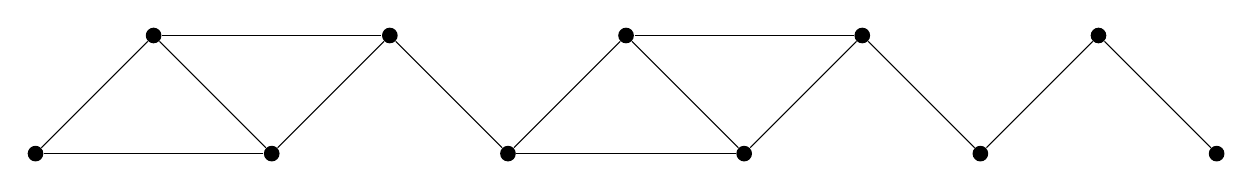
\begin{tikzpicture}[scale=1.5]
    % Define nodes
    \node (A) at (0,0) [circle,fill,inner sep=2pt] {};
    \node (B) at (1,1) [circle,fill,inner sep=2pt] {};
    \node (C) at (2,0) [circle,fill,inner sep=2pt] {};
    \node (D) at (3,1) [circle,fill,inner sep=2pt] {};
    \node (E) at (4,0) [circle,fill,inner sep=2pt] {};
    \node (F) at (5,1) [circle,fill,inner sep=2pt] {};
    \node (G) at (6,0) [circle,fill,inner sep=2pt] {};
    \node (H) at (7,1) [circle,fill,inner sep=2pt] {};
    \node (I) at (8,0) [circle,fill,inner sep=2pt] {};
    \node (J) at (9,1) [circle,fill,inner sep=2pt] {};
    \node (K) at (10,0) [circle,fill,inner sep=2pt] {};
    
    % Draw edges
    \draw (A) -- (B);
    \draw (B) -- (C);
    \draw (C) -- (D);
    \draw (D) -- (E);
    \draw (E) -- (F);
    \draw (F) -- (G);
    \draw (G) -- (H);
    \draw (H) -- (I);
    \draw (I) -- (J);
    \draw (J) -- (K);
    
    % Optional: Draw additional edges for the diamond shape
    \draw (A) -- (C);
    \draw (B) -- (D);
    \draw (E) -- (G);
    \draw (F) -- (H);
\end{tikzpicture}

\end{document}